%!TEX root = ../Thesis.tex
% \acresetall
\chapter{Classification of sleep disorders}\label{chap:classification-sleep-disorders}
% \begin{flushright}{\slshape 
%         Nobody gets it. Nothing you think matters matters. This isn't special, this is happening infinite times across infinite realites.} \\ \medskip
%         --- Rick Sanchez\\Rick and Morty, season 3, episode 10
% \end{flushright}
\begin{flushright}{\slshape 
        Break the cycle, Morty. Rise above. Focus on science.} \\ \medskip
        --- Rick Sanchez\\Rick and Morty, season 1, episode 9
\end{flushright}
\vspace{6cm}

This chapter aims to build upon the knowledge and methods introduced previously by applying them in a clinical setting.
Specifically, I will describe how we applied one of the sleep stage classification algorithms introduced in~\cref{chap:sleep-stage-classification} to identify patients with narcolepsy, which is a sleep disorder characterized by a dysfunctional regulation of the sleep-wake switch described in~\cref{sec:control-sleep}.

The content of this chapter is based on the original publication  
\begin{displayquote}
    \fullcite{Stephansen2018}\footnote{Creative Commons Attributes 4.0 International License: \url{http://creativecommons.org/licenses/by/4.0/}}
\end{displayquote}

\section{Research background}

Sleep disorders and sleep dysregulation impact over \num{100} million Americans by contributing to a range of cardiovascular, metabolic and psychiatric disorders, such as obesity, diabetes, and depression. 
Generalized sleep deprivation also negatively impairs performance, judgment, and mood, and is a major preventable contributor to motor-vehicle-related accidents~\cite{Findley1988}.
There are approximately 90 different sleep disorders currently recognized and described in the \ac{ICSD} grouped into six categories: insomnias, circadian rhythm sleep-wake disorders, central hypersomnias (\eg narcolepsy), sleep-related breathing disorders (\eg obstructive sleep apnea), parasomnias (\eg sleepwalking, \ac{RBD}), and sleep-related movement disorders (\eg \ac{PLMD} and restless legs syndrome)~\cite{AmericanAcademyofSleepMedicine2014}.%\graffito{The prevalences of insomnia, sleep apnea, and restless legs syndrome are estimated to be approximately \SIlist{20;10;4}{\percent} of the population, respectively.}, sleep apnea, restless legs syndrome, \ac{RBD}, and hypersomnia syndromes such as \ac{NT1}~\cite{AmericanAcademyofSleepMedicine2014}.

Among these pathologies, \ac{NT1} is unique as a disorder with a known, discrete pathophysiology---a destruction of hypocretin neurons in the hypothalamus, which is most likely of autoimmune origin~\cite{Peyron2000, Mignot2002, Kornum2020}.
This is reflected in the \ac{CSF} concentrations of the hypocretin-1 neuropeptide\graffito{Hypocretin-1 is also known as orexin-A.}, where a concentration below \SI{110}{\pico\gram\per\milli\liter} is considered indicative of narcolepsy~\cite{AmericanAcademyofSleepMedicine2014}\graffito{Although debated, there is also a narcolepsy type 2, which does not exhibit low \ac{CSF} hypocretin levels~\cite{Fronczek2020}.}. 

Typically beginning in childhood or adolescence, narcolepsy affects approximately \SI{0.03}{\percent} of the US, European, Korean and Chinese populations~\cite{Kornum2017}.
Unique to narcolepsy is the extremely strong association with the genetic marker \hla~\cite{Han2014}, and a well-characterized set of sleep disturbances that include short sleep latency, rapid transitions into \ac{REM} sleep and poor nocturnal sleep consolidation.
The pathology also includes episodes of \textit{sleep-wake dissociations}, where the neuron groups in the sleep-wake or \ac{REM}-\ac{NREM} switches fire at the wrong time.
This results in the clinical manifestations shown with parentheses in~\cref{fig:clinical-background:flipflop}.
% For example, experiencing REM sleep muscle paralysis while awake (sleep paralysis, cataplexy) or dreaming while awake (hypnagogic hallucinations)\todo{Revision. When this happens in NREM it results in ... etc.}.
\begin{figure}[t]
    \begin{adjustwidth*}{}{-\marginparwidth-\marginparsep}
        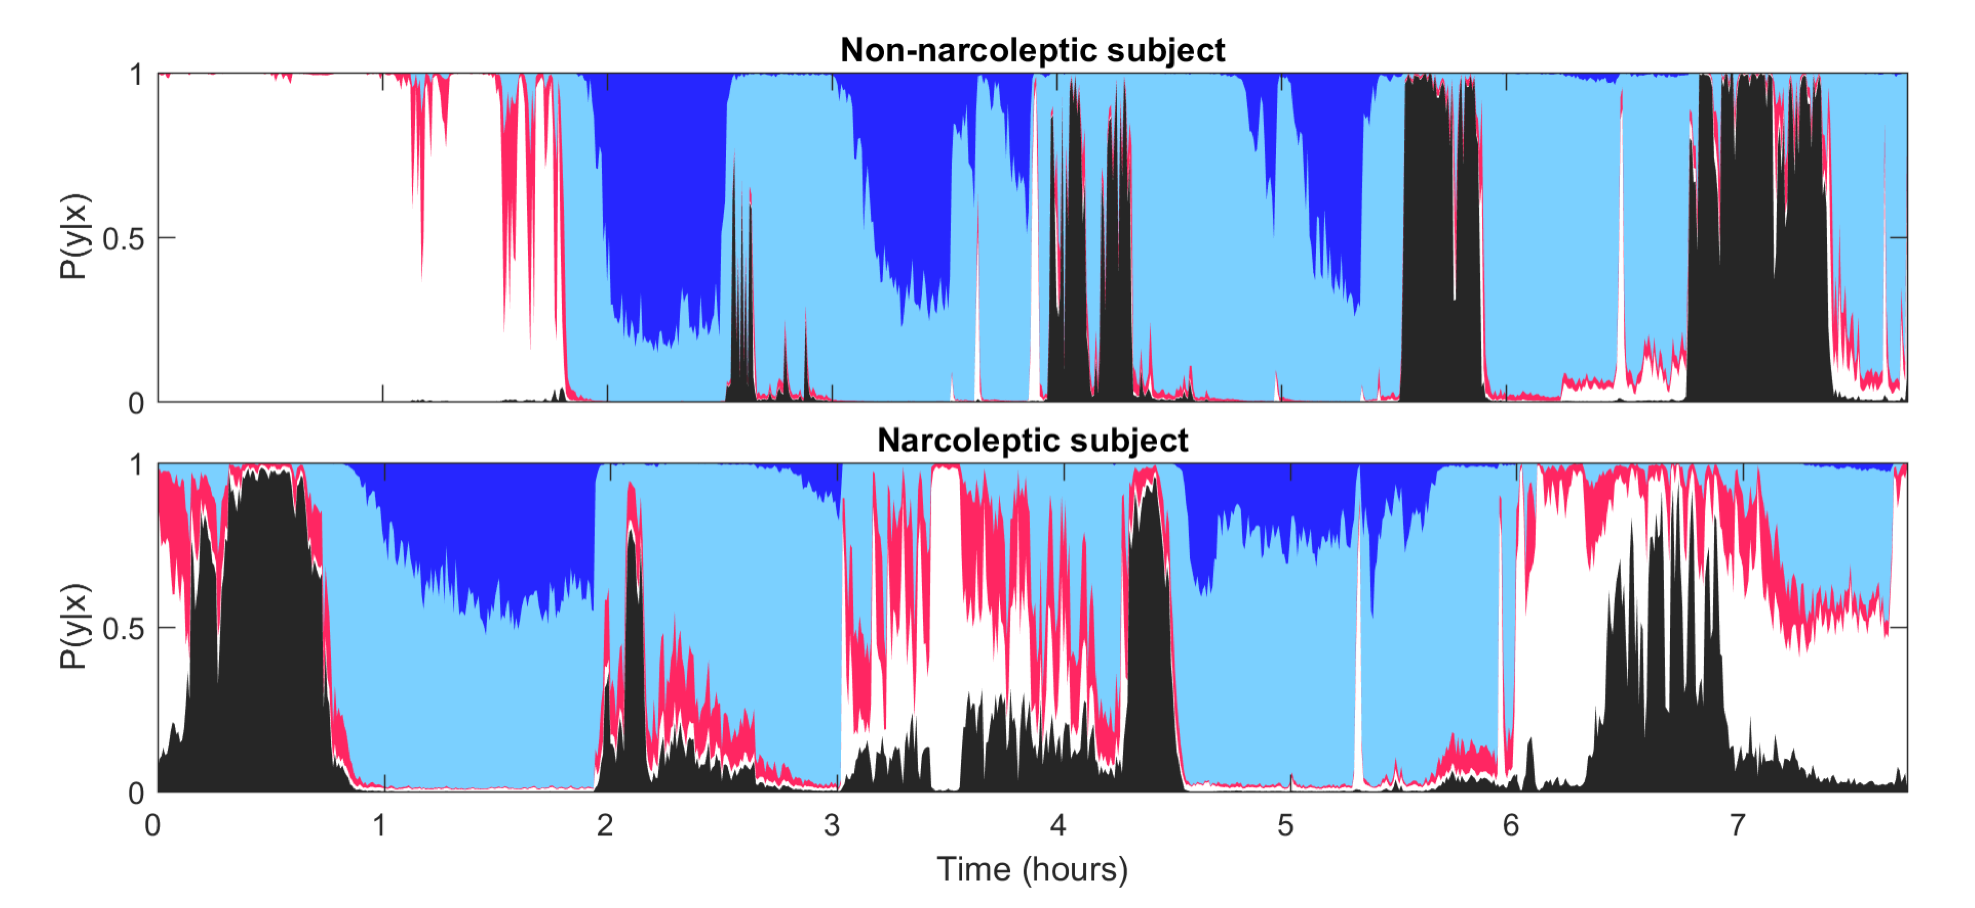
\includegraphics[width=\textwidth+\marginparwidth+\marginparsep]{figures/paper-iii/Figure_3.png}
        \caption[Examples of hypnodensity graphs.]{Examples of hypnodensity graph in subjects with and without narcolepsy. 
        Hypnodensity for a subject without narcolepsy (top) and a subject with narcolepsy (bottom). 
        Color codes: white, \ac{W}; red, \ac{N1}; light blue, \ac{N2}; dark blue, \ac{N3}; black, \ac{REM}.}
        \label{fig:paperiii-figure03}
    \end{adjustwidth*}
\end{figure}

The differentiation of sleep stages is also particularly important for the diagnosis of narcolepsy.
Current diagnostic guidelines for \ac{NT1} require a full-night \ac{PSG} and a \ac{MSLT} the following day, where patients are asked to nap \numrange{4}{5} times for \SI{20}{\minute} every \SI{2}{\hour} during the daytime, and for each nap, the sleep latency and \ac{REM} latency are noted~\cite{Littner2005}.
A \ac{MSL} less than \SI{8}{\minute}\graffito{A \ac{MSL} less than \SI{8}{\minute} is indicative of excessive sleepiness} and the presence of at least \num{2} \acp{SOREMP}\graffito{A \ac{SOREMP} is defined as \ac{REM} latency less than \SI{15}{\minute} following sleep onset in a nap.} during the \ac{MSLT}, or \num{1} \ac{SOREMP} plus a \ac{REM} latency less than \SI{15}{\minute} during nocturnal \ac{PSG} are diagnostic criteria for \ac{NT1}~\cite{AmericanAcademyofSleepMedicine2014}.
In a recent large study of the \ac{MSLT}, specificity and sensitivity for \ac{NT1} were \SIlist{98.6;92.9}{\percent} in comparing \num{516} \ac{NT1} versus \num{516} controls, respectively; and \SIlist{71.2;93.4}{\percent} in comparing \num{122} \ac{NT1} cases versus \num{132} other hypersomnia cases, respectively~\cite{Andlauer2013}.
Similar sensitivities of \SIrange{75}{90}{\percent} and specificities of \SIrange{90}{98}{\percent} have been reported by others in large samples of hypersomnia cases versus \ac{NT1}~\cite{Mignot2002,Andlauer2012,Luca2013,Dauvilliers2004,Moscovitch1993}. 
The \ac{MSLT} is thus both highly specific and highly sensitive, making it incredibly valuable as a diagnostic tool. 

\subsection{Research motivation and objectives}

In \cref{sec:paperiii}, we saw how a sleep stage classification algorithm could be constructed to reliably classify sleep stages as well or better than human experts.
The results presented an interesting observation: sleep stage classification performance was unperturbed by existing sleep disorders, except in patients with narcolepsy.
Furthermore, when comparing the hypnodensities in patients with and without narcolepsy, the former exhibited a much more diffuse sleep architecture with less pronounced sleep-wake cycles and increased \ac{REM}/\ac{W}/\ac{N1} disassociation. 
This is illustrated in~\cref{fig:paperiii-figure03} where the bottom (top) trace shows a hypnodensity graph for a subject with (without) narcolepsy.

These findings motivated a novel research question with is directly associated with research hypothesis~\ref{hypothesis:sleep-disorders}\graffito{\ref{hypothesis:sleep-disorders}: \hypothesis\xspace sleep disorders.}: 
\newcommand{\questionSleepDisorders}{based on a single overnight \ac{PSG} recording, is it possible to diagnose narcolepsy with the same level of performance as the current clinical gold standard?}
\begin{enumerate}[label={\footnotesize\bfseries\scshape RQ~3.\arabic*}, ref={\bfseries\scshape RQ~3.\arabic*}]
    \item \questionSleepDisorders\label{question:sleep-disorders}
\end{enumerate}
% \begin{displayquote}
%     based on a single overnight \ac{PSG} recording, can we diagnose narcolepsy with the same level of performance as the current clinical gold standard?
% \end{displayquote}

Derived from the research hypothesis and associated question, the following objectives were formulated:

\begin{enumerate}[label=(\roman*)]
    \item the model should be capable of diagnosing narcolepsy from the hypnodensity representation of a \ac{PSG} study;
    \item the model should have comparable or higher level of performance as the gold standard \ac{PSG}-\ac{MSLT} combination.
\end{enumerate}

The following sections describe the steps taken to complete the posed objectives and answer the research question.

% Research papers
\cleardoublepage\sectionmark{Stephansen \& Olesen, \textit{et al.}, 2018}
\section{Paper III: Neural network analysis of sleep stages enables efficient diagnosis of narcolepsy}\label{sec:paperiii-narcolepsy}
\sectionmark{Stephansen \& Olesen, \textit{et al.}, 2018}


\subsection{Methods}

The following sections will describe the narcolepsy model aspects in detail from initial hypnodensity computation, feature engineering, and finally data modeling using \ac{GP} classification algorithms.
The main outcome of this approach is to be able to classify a hypnodensity representation of a \ac{PSG} as either being positive or negative for \ac{NT1}.

\subsubsection{Model overview}

The general pipeline for training and testing the narcolepsy model is shown in~\cref{fig:paperiii-figure5c}.
On the left side is shown the input data sources from the cohorts described in~\cref{tab:paperiii-supptable01}.
The \acp{PSG} from these cohorts are extracted and subjected to the sleep stage scoring model described in~\cref{sec:paperiii} resulting in a hypnodensity\graffito{The hypnodensity is further described in~\cref{sec:paperiii}, but is essentially a probability distribution over sleep stages.} representation for the \textit{i}th \ac{PSG}.

The hypnodensity data are split into training and testing subsets in a \SI{60}{\percent}/\SI{40}{\percent} ratio.
The training data are used for building the \ac{GP} narcolepsy model with a subset of features determined using a feature reduction agorithm.
Cross-validation was employed to determined the optimal classification threshold, and the performance of the classifier was determined on the held-out testing data.

\begin{figure}
    % \centering
    \begin{adjustwidth*}{}{-\marginparwidth-\marginparsep}
        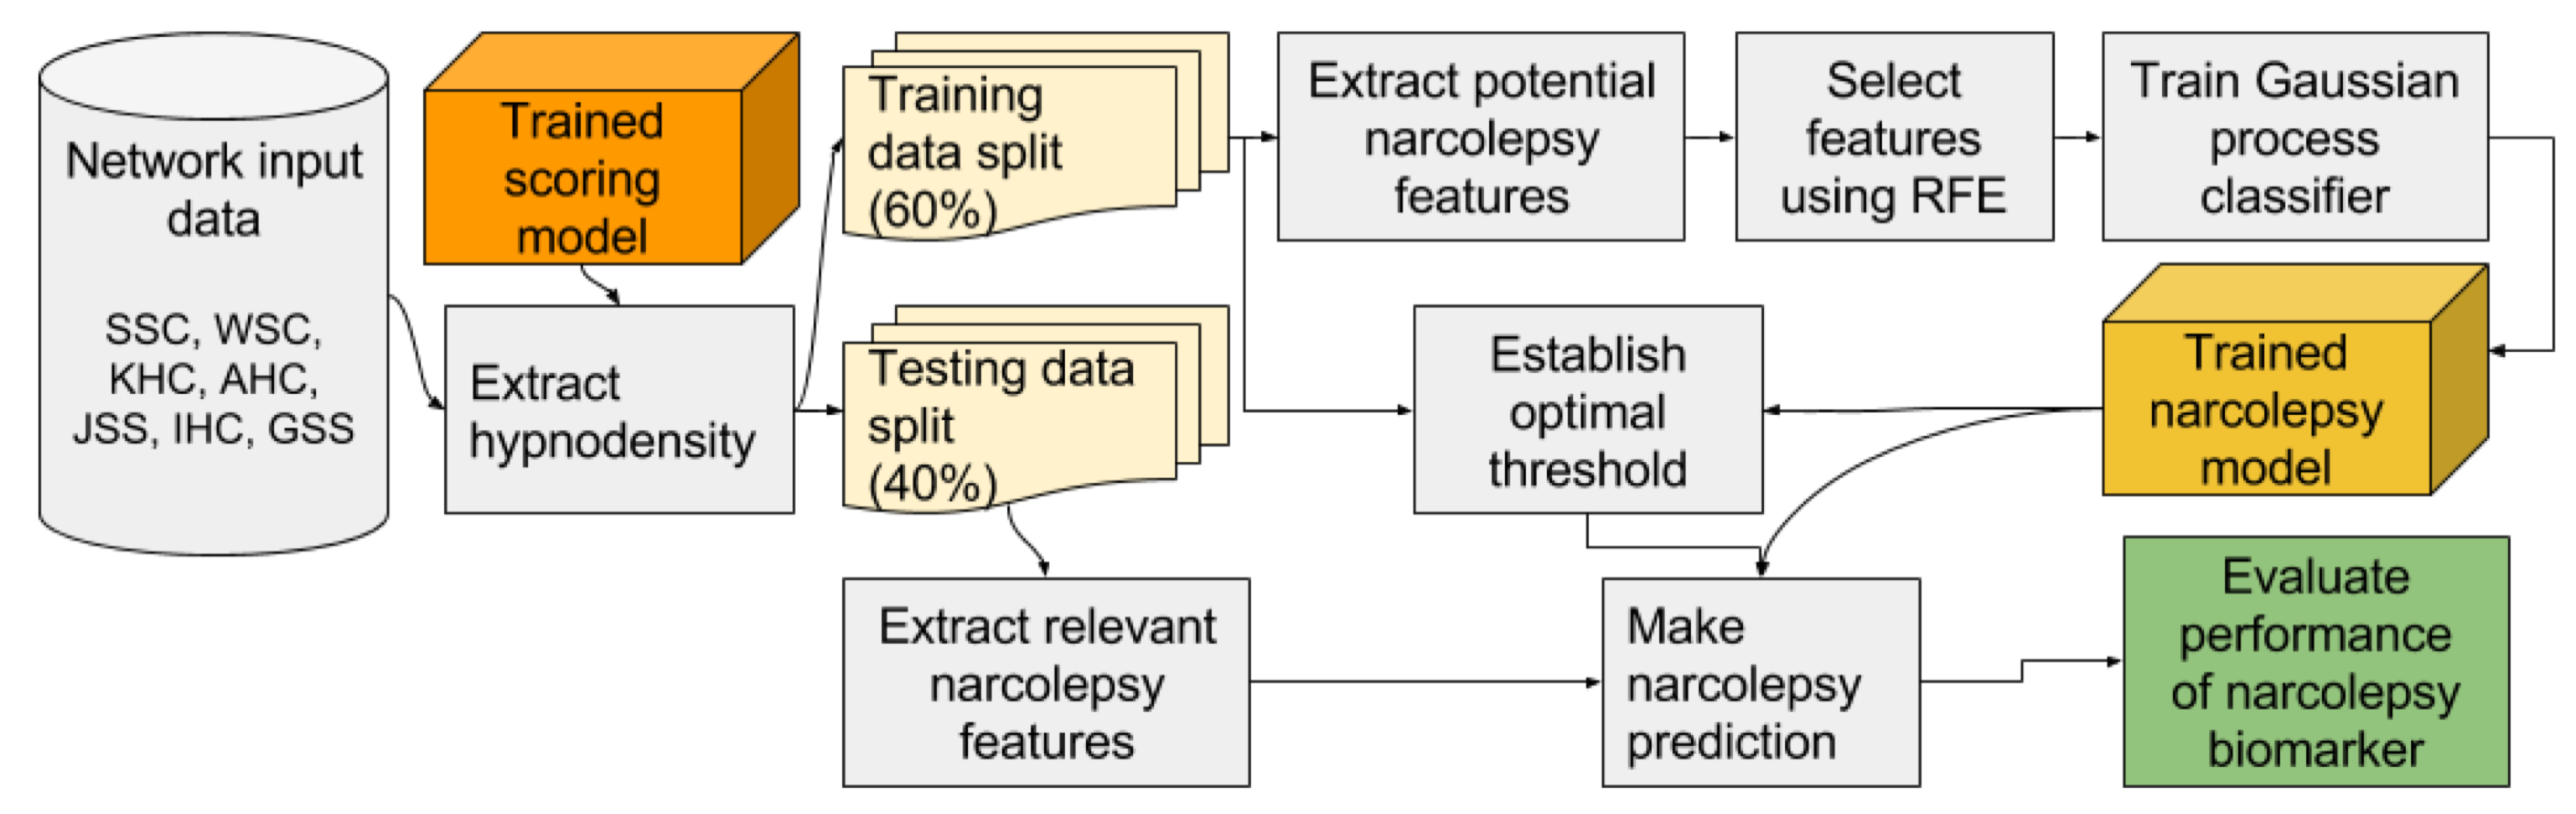
\includegraphics[width=\textwidth+\marginparwidth+\marginparsep]{figures/paper-iii/Figure_5c.png}
        \caption[Narcolepsy detector algorithm design]{Narcolepsy detector algorithm design. Hypnodensities are extracted from data, as described in~\cref{sec:paperiii}. 
        These data are separated into a training (\SI{60}{\percent}) and a testing (\SI{40}{\percent}) split. 
        From the training split, 481 potentially relevant features described in~\cref{tab:paperiii-supptable10} are extracted from each hypnodensity. 
        The prominent features are selected using a \ac{RFE} algorithm, and the narcolepsy detection model is trained using a \ac{GP} model.
        The performance of the \ac{GP} narcolepsy detection  model is evaluated using the selected features computed on the test data.}
        \label{fig:paperiii-figure5c}
    \end{adjustwidth*}
\end{figure}

\subsubsection{Feature extraction for \ac{NT1}}

The following sections describe the features computed for each hypnodensity representation.
Overall, the features fall into two categories:
\begin{enumerate*}[label={(\roman*)}]
\item features based on the dynamics between various stage combinations; and,
\item features based on reported findings in the literature.
\end{enumerate*}

\paragraph{Hypnodensity-derived features}
To quantify narcolepsy-like behavior for a single recording \textit{i}, features were generated based on a proto-feature derived from \textit{k}-combinations of $\mathcal{S} = \lbrace \wake, \rem, \nI, \nII, \nIII \rbrace$. 
For the \textit{n}th \num{5}, \num{15} or \SI{30}{\second} segment in recording \textit{i}, a single \textit{k}-combination is selected from the set of all \textit{k}-combinations, and the proto-feature is then calculated as the sum of the pair-wise products of the elements in the single \textit{k}-combination, such that
\begin{equation}
    \boldsymbol{\Phi}^{(i)}_{n} \! \! \left( \mathcal{S}_{k} \right) = \sum_{\zeta \in \lbrack \mathcal{S}_{k} \rbrack^2} \prod_{s \in \zeta}{p\!\left( \! s \! \mid \! \mathbf{x}_{n}^{(i)} \! \right)}, \quad p \in \lbrack 0,1 \rbrack,
\end{equation}
where $\boldsymbol{\Phi}^{(i)}_{n}$ is the proto-feature for the \textit{n}th segment in recording \textit{i}, $\zeta \in \lbrack \mathcal{S}_{k} \rbrack^2$ is a \num{2}-tuple, or pair-wise combination, in the set of all pair-wise combinations in the \textit{k}-combination of $\mathcal{S}$, and $s$ is a single element, or sleep stage, in $\zeta$.
For $k \in \llbracket 5 \rrbracket$, there are 31 different $\mathcal{S}_k$, e.g. $\lbrace \wake, \rem \rbrace, \lbrace \nI, \nII, \nIII \rbrace$.
The predicted probability of a 5, 15 or \SI{30}{\second} epoch belonging to a certain class in $\mathcal{S}$ given the data $\mathbf{x}^{(i)}_n$ is given by \( p\!\left( \! s \! \mid \! \mathbf{x}_{n}^{(i)} \! \right) \).
For every value of \textit{k}, 15 features based on the mean, derivative, entropy and cumulative sum were extracted as shown in~\cref{tab:paperiii-supptable10}.

\begin{table}[t]
\begin{adjustwidth*}{}{}
\small
\renewcommand{\arraystretch}{1.2}
\begin{threeparttable}
    \caption[Description of narcolepsy features]{Description of each feature, how it is calculated, and how it is numerated.}
    \label{tab:paperiii-supptable10}
    \begin{tabular}{@{}llc@{}} \toprule
        \textbf{\#} & \textbf{Description} & \textbf{Formula} \\ \midrule
        \num{1} & General prevalence of a value & \( \log \! \parenthesis{\frac{1}{N} \sum_{n=1}^{N}{\boldsymbol{\Phi}_{n} \! \! \parenthesis{\mathcal{S}_{k}}}} \) \\
        \num{2} & Highest achieved value & \( -\log \! \parenthesis{1 - \max{\boldsymbol{\Phi}_{n} \! \! \parenthesis{\mathcal{S}_{k}}}} \) \\
        \num{3} & Average fluctuations in value & \( \log \! \parenthesis{ \frac{1}{N} \sum_{n=1}^{N}{ \mid \frac{ \mathrm{d} \boldsymbol{\Phi}_{n} \! \! \parenthesis{\mathcal{S}_{k}} }{ \mathrm{d} n } \mid }} \) \\
        \num{4} & Log of Shannon entropy & \( \log \! \parenthesis{ \frac{-\sum_{i} s_{i}^{2} \log s_{i}^{2}}{N} } \) \\
        \numrange[range-phrase = --]{5}{8} & Time until \textit{p} times max. value & \( \log \! \parenthesis{\mathrm{first}_{p} \! \parenthesis{ \frac{ \mathrm{cum \, sum \! \parenthesis{ \boldsymbol{\Phi} \! \! \parenthesis{\mathcal{S}_{k}} }} }{ \mathrm{sum} \! \parenthesis{ \boldsymbol{\Phi} \! \! \parenthesis{\mathcal{S}_{k}} } } } \times 30} \) \\
        \num{9} & Weighted maximum & \( \sqrt{\max{ \boldsymbol{\Phi} \! \! \parenthesis{\mathcal{S}_{k}} } \times \bar{ \boldsymbol{\Phi}} \! \! \parenthesis{\mathcal{S}_{k}} } \) \\
        \num{10} & Weighted average fluctuation & \( \parenthesis{ \frac{1}{N} \sum_{n=1}^{N}{ \mid \frac{ \mathrm{d} \boldsymbol{\Phi}_{n} \! \! \parenthesis{\mathcal{S}_{k}} }{ \mathrm{d} n } \mid }} \times \bar{ \boldsymbol{\Phi}} \! \! \parenthesis{\mathcal{S}_{k}} \) \\
        \num{11} & Weighted Shannon entropy & \( \log \! \parenthesis{ \frac{-\sum_{i} s_{i}^{2} \log s_{i}^{2}}{N} \times \bar{ \boldsymbol{\Phi}} \! \! \parenthesis{\mathcal{S}_{k}} } \) \\
        \numrange[range-phrase = --]{12}{15} & Weighted time until \textit{p} max value & \( \sqrt{ \log \! \parenthesis{\mathrm{first}_{p} \! \parenthesis{ \frac{ \mathrm{cum \, sum \! \parenthesis{ \boldsymbol{\Phi} \! \! \parenthesis{\mathcal{S}_{k}} }} }{ \mathrm{sum} \! \parenthesis{ \boldsymbol{\Phi} \! \! \parenthesis{\mathcal{S}_{k}} } } } \times 30} } \) \\
        \bottomrule
    \end{tabular}
    \begin{tablenotes}
        \small
        \item[4] The Shannon entropy is calculated using wavelet decompositions of \( \boldsymbol{\Phi} \! \! \parenthesis{\mathcal{S}_{k}} \), where \(s_i\) contains the \textit{i}th detail coefficient. This feature describes the amount of information contained in the signal.
        \item[5--8] \textit{p} here corresponds to \SIlist{5;10;30;50}{\percent}. 
        \item[12--15] \textit{p} here corresponds to \SIlist{5;10;30;50}{\percent}. 
        \item Each individual feature is scaled by subtracting the mean and dividing by the difference between the \nth{85} and \nth{15} percentile values.
        Each value was assessed visually to ensure that the transformations and scaling was done optimally.
        \( \mathrm{cum \, sum} \) is the cumulative sum.
    \end{tablenotes}
\end{threeparttable}
\end{adjustwidth*}
\end{table}

\paragraph{Additional \ac{PSG} features}
In addition to the features described above, another set of features reflecting abnormal sleep stage sequencing in \ac{NT1} was investigated.

One set of such features was selected because they have been found to differentiate \ac{NT1} from other subjects in prior studies~\cite{Christensen2015a,Roth2013,Hansen2017,Drakatos2013,Liu2015b}. 
These include
\begin{itemize}
    \item nocturnal \ac{REML}~\cite{Andlauer2013},
    \item presence of a nightly \ac{SOREMP} with a \ac{REML} less than \SI{15}{\minute}~\cite{Andlauer2013},
    \item presence and number of \acp{SOREMP} during the night, where the \acp{SOREMP} are defined as \ac{REM} sleep occurring after at least \SI{2.5}{\minute} of either \ac{W} or \ac{N1}, and
    \item nocturnal sleep latency~\cite{Christensen2015a}\graffito{A short sleep latency is common in patients with \ac{NT1}}.
\end{itemize}
Other features include 
\begin{itemize}
    \item a \ac{NREM} fragmentation index defined as 22 or more occurrences, where sustained \ac{N2}/\ac{N3} is broken by at least \SI{1}{\minute} of \ac{N1}/\ac{W}~\cite{Christensen2015a}, and
    \item the number of \ac{W}/\ac{N1} hypnogram bouts longer than \SI{3}{\minute}~\cite{Christensen2015a}.
\end{itemize}

In this study we also explore: 
\begin{itemize}
    \item the cumulative \ac{W}/\ac{N1} duration for wakefulness periods shorter than \SI{15}{\minute};
    \item cumulative \ac{REM} duration following \ac{W}/\ac{N1} periods longer than \SI{2.5}{\minute}; and,
    \item total nightly \ac{SOREMP} duration defined as the sum of \ac{REM} epochs following \SI{2.5}{\minute} \ac{W}/\ac{N1} periods.
\end{itemize}

% Another set of nine features reflecting the hypnodensity sleep stage distribution was defined based on the peakedness of the accumulation of sleep stages, as noted in~\cref{fig:paperiii-suppfigure04}. 
% These features based on the order of the peaks, expressing a type of transition (\wake{} to \nI{}, \wake{} to \rem{}, \rem{} to \nIII{} etc.). 
% If the height of the \textit{n}th peak is denoted as $\phi_n$, the transition value $\tau$ is calculated as the geometric mean between successive peaks:
% \begin{equation}
%     \tau = \sqrt{\phi_n \phi_{n+1}}
% \end{equation}
% Due to their likeness, \wake{} and \nI{} peaks were added to form a single type.
% All transitions of a certain type were added together to form a single feature. A lower limit of 10 was imposed on peaks to avoid spurious peaks. If two peaks of the same type appeared in succession the values were combined into a single peak.


\subsubsection{Probabilistic models for diagnostic purposes} 
The large set of features was reduced using a cross-validated \ac{RFE} algorithm~\cite{Guyon2002}.
Using a threshold of 0.40 yielded 38 relevant features, which were fed to a \ac{GP} classifier as described below.
GP classifiers are non-parametric probabilistic models that produce robust non-linear decision boundaries using kernels\graffito{Gaussian processes can also be viewed as a probabilistic extension of support vector machines.} and provide estimates of the uncertainities in classifications.
This is useful when combining estimates, but also when making a diagnosis; if an estimate is particularly uncertain, a doctor may opt for more tests to increase certainty before making a diagnosis.
During \ac{GP} model building, a training dataset is used to optimize a set of hyper-parameters, which specify the kernel function, the basis function coefficients, here a constant, noise variance, and to form the underlying covariance and mean function from which inference about new cases are made~\cite{Rasmussen2006}.
In this case, the kernel is the squared exponential:
Two classes were established: narcolepsy type 1 and “other”, which contains every other subject.
These were labeled 1 and -1 respectively, placing all estimates in this range.
For more information on GP in general, see the textbook by \citeauthor{Rasmussen2006}\cite{Rasmussen2006}, while more information on variational inference for scalable \ac{GP} classification can be found in the paper by \citeauthor{Hensman2015}\cite{Hensman2015} and by \citeauthor{Matthews2017}\cite{Matthews2017}.

\paragraph{HLA testing}
As described previously, \SI{97}{\percent} of \ac{NT1} patients are \hla positive when the disease is defined biochemically by low \ac{CSF} hypocretin-1, or by the presence of cataplexy coupled with clear \ac{MSLT} findings~\cite{Han2014,Andlauer2013}. 
We implemented this feature as a binary-valued predictor resulting in negative narcolepsy predictions for subjects with a negative \hla test result.

\paragraph{High pretest probability sample}
\Acp{MSLT} are typically performed in patients with daytime sleepiness that cannot be explained by \ac{OSA}, insufficient sleep or circadian disturbances alone. 
These patients thus have a higher pre-test probability of having \ac{NT1} than random clinical patients and are then diagnosed with \ac{NT1} or \ac{NT2}, idiopathic hypersomnia or subjective sleepiness based on \ac{MSLT} results, cataplexy symptoms and \ac{HLA} results, if they are available.
To test whether our detector differentiates \ac{NT1} from these other cases with unexplained sleepiness, we conducted a post-hoc analysis of the detector performance in these subjects extracted from both the test and replication datasets.

\subsection{Results}

The neural networks produce outputs that depend on evidence in the input data for or against a certain sleep stage based on features learned through training.
We hypothesized that narcolepsy, a condition characterized by sleep/wake stage mixing/ dissociation~\cite{Christensen2015a,Olsen2017,Jensen2014,Vassalli2013,Pizza2015}, would result in a greater than normal overlap between stages, such as that shown in~\cref{fig:paperiii-figure03}.
Based on this result, we hypothesized that such sleep stage model outputs could be used as a biomarker for the diagnosis of \ac{NT1} using a standard nocturnal \ac{PSG} rather than the \ac{PSG}-\ac{MSLT} combination.

To quantify narcolepsy-like behavior for a single recording, we generated features quantifying sleep stage mixing/dissociation. 
These are based on descriptive statistics and other features describing persistence of a set of new time series generated from the geometric mean of every permutation of the set of sleep stages, as obtained from the 16 sleep stage prediction models.

In addition to this, we also added features expected to predict narcolepsy based on prior work, such as \ac{REM} sleep latency and sleep stage sequencing parameters. 
A \ac{RFE} procedure was performed on extracted features with average outcome setting the optimal number of relevant features at 38~\cite{Guyon2002}. 

\begin{table}
    % \centering
    % \begin{adjustwidth*}{}{-\marginparwidth-\marginparsep}
    \small
    \caption[Narcolepsy features selection frequencies]{Selection frequency and descriptions of each of the 38 features included in the \acl{GP} model used for narcolepsy prediction. Numbers in second column correspond to feature number in~\cref{tab:paperiii-supptable10}.}
    \label{tab:paperiii-supptable05}
    % \begin{tabular}{@{}lp{4.5cm}lp{2.5cm}@{}}
    \begin{tabular}{@{}lp{6cm}lr@{}}
        \toprule
           & Feature                                                & Stage combination  & Frequency \\ \midrule
        1  & 12                                                     & \ac{W}, \ac{N2}, \ac{REM}             & 1.00                         \\
        2  & \multicolumn{2}{l}{Nightly \acp{SOREMP}}                                                       & 0.91                         \\
        3  & 15                                                     & \ac{W}                                & 0.82                         \\
        4  & 6                                                      & \ac{REM}                              & 0.82                         \\
        5  & 2                                                      & \ac{W}                                & 0.68                         \\
        6  & 2                                                      & \ac{N2}, \ac{REM}                     & 0.68                         \\
        7  & 14                                                     & \ac{W}, \ac{N2}                       & 0.68                         \\
        8  & 13                                                     & \ac{W}, \ac{N1}                       & 0.64                         \\
        9  & 5                                                      & \ac{N3}                               & 0.59                         \\
        10 & 5                                                      & \ac{REM}                              & 0.59                         \\
        11 & 13                                                     & \ac{N1}, \ac{N2}                      & 0.59                         \\
        12 & 8                                                      & \ac{N1}                               & 0.55                         \\
        13 & 11                                                     & \ac{N1}                               & 0.55                         \\
        14 & 7                                                      & \ac{W}, \ac{N1}, \ac{REM}             & 0.55                         \\
        15 & 5                                                      & \ac{W}, \ac{N1}, \ac{N3}              & 0.55                         \\
        16 & 6                                                      & \ac{W}, \ac{N1}, \ac{N3}              & 0.55                         \\
        17 & 1                                                      & \ac{W}, \ac{N1}, \ac{N2}, \ac{REM}    & 0.55                         \\
        18 & \multicolumn{2}{l}{Hypnodensity sleep stage bout transitions from \ac{N2} to \ac{N3}}          & 0.55                         \\
        19 & \multicolumn{2}{l}{Accumulation of \ac{W} periods less than \SI{15}{\minute}}                  & 0.50                         \\
        20 & \multicolumn{2}{l}{Hypnodensity sleep stage bout transitions from \ac{W}/\ac{N1} to \ac{REM}}  & 0.50                         \\
        21 & 11                                                     & \ac{N3}, \ac{REM}                     & 0.45                         \\
        22 & 2                                                      & \ac{N1}, \ac{REM}                     & 0.45                         \\
        23 & 7                                                      & \ac{W}, \ac{N2}, \ac{N3}              & 0.45                         \\
        24 & 12                                                     & \ac{W}                                & 0.41                         \\
        25 & 2                                                      & \ac{N1}                               & 0.41                         \\
        26 & 12                                                     & \ac{N2}                               & 0.41                         \\
        27 & 14                                                     & \ac{N2}                               & 0.41                         \\
        28 & 7                                                      & \ac{N2}, \ac{REM}                     & 0.41                         \\
        29 & 8                                                      & \ac{N2}, \ac{REM}                     & 0.41                         \\
        30 & 6                                                      & \ac{N1}, \ac{N2}                      & 0.41                         \\
        31 & 15                                                     & \ac{N1}, \ac{N2}                      & 0.41                         \\
        32 & 15                                                     & \ac{W}, \ac{N3}                       & 0.41                         \\
        33 & 12                                                     & \ac{W}, \ac{N1}                       & 0.41                         \\
        34 & 5                                                      & \ac{W}, \ac{N2}, \ac{REM}             & 0.41                         \\
        35 & 1                                                      & \ac{W}, \ac{N1}, \ac{N3}, \ac{REM}    & 0.41                         \\
        36 & 1                                                      & \ac{W}, \ac{N1}, \ac{N2}, \ac{N3}, \ac{REM}   & 0.41                 \\
        37 & \multicolumn{2}{l}{Accumulation of \ac{REM} epochs following \ac{W} periods}                   & 0.41                         \\
        38 & \multicolumn{2}{l}{Hypnodensity sleep stage bout transitions from \ac{N2} to \ac{REM}}         & 0.41                         \\ \bottomrule
    \end{tabular}
    % \end{adjustwidth*}
\end{table}

An optimal selection frequency cut-off of 0.40\graffito{That means including a feature if it was selected in \SI{40}{\percent} of the cross-validation runs} was determined using a cross-validation setup on the training data. 
The selected features are described in~\cref{tab:paperiii-supptable05} with detailed description of the eight most important features reported in~\cref{tab:paperiii-table04}.

Final predictions were achieved by creating a separate \ac{GP} narcolepsy classifier for each of the sleep scoring models used in the final implementation. 
This was tested in seven independent datasets: a training dataset constituted of PSG from WSC32,33, SSC10,32,KHC10,34,AHC35, Jazz Clinical Trial Sample (JCTS)43,Italian Hypersomnia Cohort (IHC)41 and DHC; with verification in test data mostly constituted of PSG from the same cohorts and independent replication in the French Hypersomnia Cohort (FHC) and the Chinese Narcolepsy Cohort (CNC)12 that had never been seen by the algorithm~\cref{tab:paperiii-supptable01}. 
The algorithm produced values between -1 and 1, with 1 indicating a high probability of narcolepsy. 
A cut-off threshold between narcolepsy type 1 and “other“ was set at -0.03 (red dot, Fig. 4), determined using training data, as shown in Fig. 4a. 
The optimal trade-off achieves both high sensitivity and specificity, which is seen to translate well onto the test data (Fig. 4b) and the never seen replication sample (Fig. 4c).

\begin{figure}
    \begin{adjustwidth*}{}{-\marginparwidth-\marginparsep}
    \myfloatalign   
    \subfloat[]
    {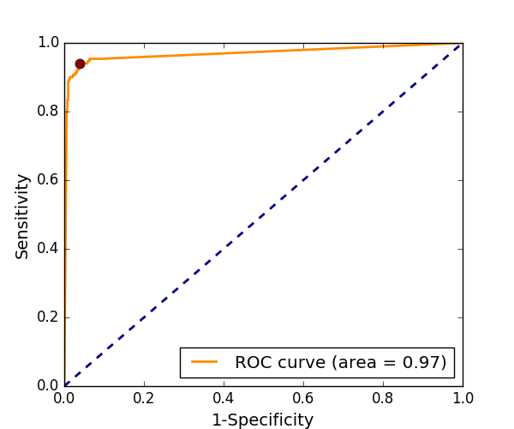
\includegraphics[width=0.5\textwidth + 0.5\marginparwidth + 0.5\marginparsep]{figures/paper-iii/Figure_4a.png}}
    \subfloat[]
    {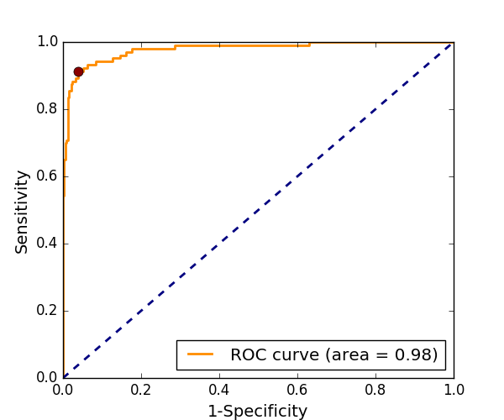
\includegraphics[width=0.5\textwidth + 0.5\marginparwidth + 0.5\marginparsep]{figures/paper-iii/Figure_4b.png}} \\
    \subfloat[]
    {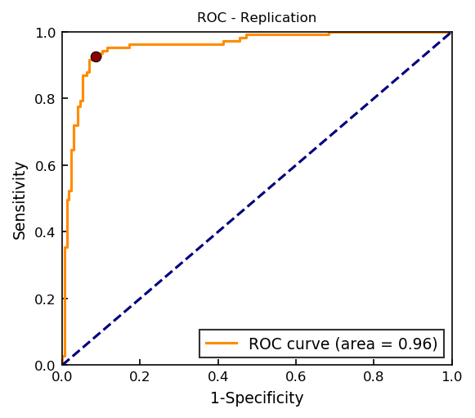
\includegraphics[width=0.5\textwidth + 0.5\marginparwidth + 0.5\marginparsep]{figures/paper-iii/Figure_4c.png}}
    \subfloat[]
    {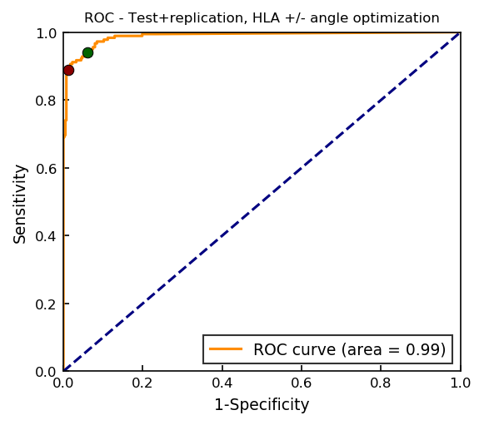
\includegraphics[width=0.5\textwidth + 0.5\marginparwidth + 0.5\marginparsep]{figures/paper-iii/Figure_4d.png}} \\
    \subfloat[]
    {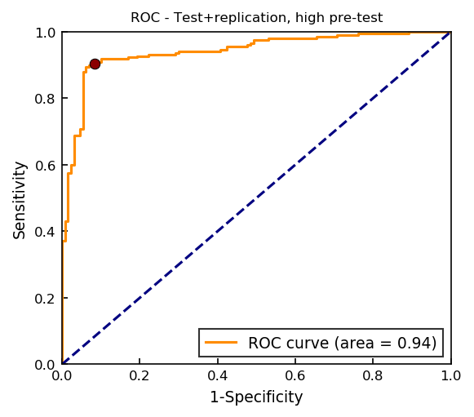
\includegraphics[width=0.5\textwidth + 0.5\marginparwidth + 0.5\marginparsep]{figures/paper-iii/Figure_4e.png}}
    \subfloat[]
    {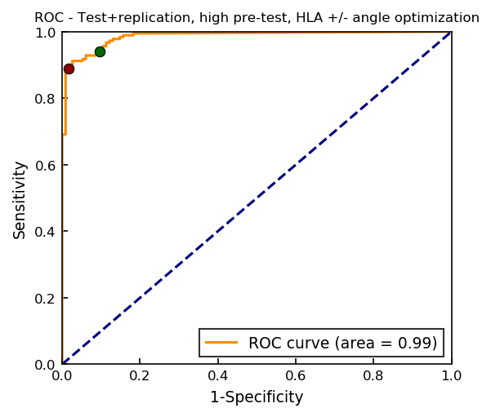
\includegraphics[width=0.5\textwidth + 0.5\marginparwidth + 0.5\marginparsep]{figures/paper-iii/Figure_4f.png}}
    \caption[Diagnostic receiver operating characteristics curves for narcolepsy model]{Diagnostic receiver operating characteristics curves for narcolepsy model displaying the trade-offs between sensitivity and specificity for the narcolepsy biomarker for (a) training sample, (b) testing sample, (c) replication sample, and (e) high pretest sample. 
    (d)–(f) Adding \ac{HLA} to model greatly increases specificity. 
    Cut-off thresholds are presented for models with (red dot) and without \ac{HLA} (green dot)}
    \label{fig:paperiii-figure04}
    \end{adjustwidth*}
\end{figure}

In the training data, a sensitivity of \SI{94}{\percent} and specificity of
\SI{96}{\percent} was achieved, and in the testing data a sensitivity of \SI{91}{\percent} and specificity of \SI{96}{\percent} was achieved, while the sensitivity and specificity for the replication sample was \SIlist{93;91}{\percent}, respectively. 
When \ac{HLA} was added to this model (\cref{fig:paperiii-figure04}d--f), the sensitivity changed to \SI{90}{\percent} and the specificity rose to \SI{99}{\percent}, and the cut-off threshold was updated to \num{-0.53} shown with green dots in~\cref{fig:paperiii-figure04}d--f.
Furthermore, in the high pretest sample we obtained a sensitivity and specificity of \SIlist{90;92}{\percent}, which rose to \SIlist{90;98}{\percent} when adding \ac{HLA}.
More descriptive statistics including \SI{95}{\percent} confidence intervals are shown in~\cref{tab:paperiii-supptable06}.

\begin{table}
    % \centering
    \small
    \begin{adjustwidth*}{}{-\marginparwidth-\marginparsep}
    \caption{Eight most frequently selected features for \ac{NT1} detection.}
    \label{tab:paperiii-table04}
    % \begin{tabular*}{\textwidth+\marginparwidth+0.5\marginparsep}{@{}lcp{\textwidth}@{}}
    \begin{tabular}{@{}lcp{\marginparsep+\textwidth}@{}}
        \toprule
          & Frequency & Description \\
        \midrule
        1 & 1.00 & Time until \SI{5}{\percent} of the weighted sum of the product between \acs{W}, \acs{N2}, and \acs{REM} calculated at every epoch has accumulated. This feature expresses the known sleep stage dissociation and altered sleep timing.\\
        2 & 0.91 & Number of \acp{SOREMP} appearing throughout the recording.\\
        3 & 0.82 & Time until \SI{50}{\percent} of \ac{W} in recording has accumulated weighted by total amount of \ac{W}.\\
        4 & 0.82 & Shannon entropy of \ac{REM} sleep. This expresses the amount of information held in a signal, or in this case, how many different values the \ac{REM} sleep stage distribution obtains, \ie how consolidated phases of \ac{REM} are when the stage appears. \\
        5 & 0.68 & Maximum probability of \ac{W} obtained in a recording. \\
        6 & 0.68 & Naximum value obtained of the product between \ac{N2} and \ac{REM} probability in a recording.\\
        7 & 0.68 & Time until \SI{30}{\percent} of the epoch-by-epoch sum product between \ac{W} and \ac{N2} has accumulated, weighted by the sum total. \\
        8 & 0.64 & The time taken before \SI{10}{\percent} of the epoch-by-epoch sum product between \ac{W} and \ac{N1} has accumulated, weighted by the sum total.\\
        \bottomrule
    \end{tabular}
    \end{adjustwidth*}
\end{table}

\begin{table}
    % \centering
    \small
    \begin{adjustwidth*}{}{-\marginparwidth-\marginparsep}
    \caption[Narcolepsy biomarker performance]{Descriptive statistics on the evaluation of the narcolepsy biomarker in models with and without the \ac{HLA} biomarker. 
    Performance on models with \ac{HLA} typing is reported for both regular and optimized threshold, since the \ac{ROC} curve changes by adding \ac{HLA}. Mean value and 95\% confidence interval.}
    \label{tab:paperiii-supptable06}
    \begin{tabular}{@{}llllllrr@{}}
        \toprule
        \textbf{Model}      & \textbf{Accuracy}, \% & \textbf{Sensitivity}, \% & \textbf{Specificity}, \% & \textbf{PPV}, \%  & \textbf{NPV}, \%  & \textbf{\acp{PSG}} & \textbf{\ac{NT1}}, \% \\ \midrule
        T                   & 0.95          & 0.91             & 0.96             & 0.88      & 0.97      & 444       & 0.24                       \\
                            & 0.92-0.97     & 0.84-0.96        & 0.93-0.98        & 0.80-0.93 & 0.95-0.99 &           &                            \\
        R                   & 0.92          & 0.93             & 0.91             & 0.87      & 0.95      & 321       & 0.28                       \\
                            & 0.88-0.95     & 0.87-0.97        & 0.87-0.95        & 0.80-0.93 & 0.92-0.98 &           &                            \\
        \multirow[t]{2}{0.175\textwidth}{T+R, HLA} & 0.96          & 0.9              & 0.99             & 0.97      & 0.95      & 584       & 0.31                       \\
                            & 0.94-0.97     & 0.84-0.93        & 0.98-1.00        & 0.94-0.99 & 0.93-0.97 &           &                            \\
        \multirow[t]{2}{0.175\textwidth}{T+R, HLA, optim.}    & 0.94          & 0.94             & 0.94             & 0.88      & 0.97      & 584       & 0.31                       \\
                            & 0.92-0.96     & 0.90-0.97        & 0.92-0.96        & 0.83-0.92 & 0.95-0.99 &           &                            \\
        \multirow[t]{2}{0.175\textwidth}{HPT, no HLA.}        & 0.91          & 0.9              & 0.92             & 0.94      & 0.86      & 335       & 0.61                       \\
                            & 0.87-0.94     & 0.86-0.94        & 0.86-0.96        & 0.91-0.97 & 0.80-0.91 &           &                            \\
        \multirow[t]{2}{0.175\textwidth}{HPT, HLA}            & 0.93          & 0.9              & 0.98             & 0.99      & 0.85      & 296       & 0.61                       \\
                            & 0.90-0.95     & 0.84-0.93        & 0.96-1.00        & 0.97-1.00 & 0.79-0.91 &           &                            \\
        \multirow[t]{2}{0.175\textwidth}{HPT, HLA, optim.}    & 0.93          & 0.94             & 0.9              & 0.94      & 0.9       & 296       & 0.61                       \\
                            & 0.90-0.95     & 0.90-0.97        & 0.85-0.95        & 0.90-0.97 & 0.85-0.95 &           &                            \\ \bottomrule
    \end{tabular}
    \end{adjustwidth*}
\end{table}

\subsection{Discussion}

Using our models, and considering how typical \ac{NT1} behaved in our sleep stage machine learning routines, we extracted features that could be useful to diagnose this condition.
\Ac{NT1} is characterized by a loss of hypocretin-producing cells in the hypothalamus and can be best diagnosed by measuring hypocretin levels in the \ac{CSF}~\cite{Peyron2000,Mignot2002}, a procedure that requires a lumbar puncture, which is rarely performed in the United States\todo{Need sources on this and in Europe}.
At the symptomatic level, \ac{NT1} is characterized by sleepiness, cataplexy\graffito{cataplexic episodes are defined by muscle weakness during wakefulness often triggered by strong emotions.} and numerous symptoms reflecting poor nocturnal sleep (insomnia) and symptoms of \textit{dissociated REM sleep}.
Dissociated \ac{REM} sleep is reflected in the hypnogram/hypnodensity by the presence of unusual states of consciousness where \ac{REM} sleep intermingles with wakefulness thus producing disturbing reports of dreams that interrupt wakefulness and seem real\graffito{this is also called hypnagogic halluciations.}, or episodes where the sleeper is awake, but paralyzed, as in normal REM sleep\graffito{this is also called sleep paralysis.}.
The current gold standard for \ac{NT1} diagnosis is the presence of cataplexy and a positive \ac{MSLT}.
In a recent large study of the \ac{MSLT}, specificity and sensitivity for \ac{NT1} was \SIlist{98.6;92.9}{\percent} in comparing \ac{NT1} versus controls, and \SIlist{71.2;93.4}{\percent} in comparing \ac{NT1} versus other hypersomnia cases~\cite{Andlauer2013}.

\Cref{tab:paperiii-table04,tab:paperiii-supptable05} reveal features found in nocturnal \acp{PSG} that discriminate \ac{NT1} and non-narcoleptics. 
One of the most prominent features, short latency \ac{REM} sleep, bears great resemblance to the \ac{REM} sleep latency, which is already used clinically to diagnose narcolepsy, although in this case it is calculated using fuzzy logic and thus represent a latency where accumulated sleep is suggestive of a high probability of \ac{REM} sleep having occurred\graffito{As opposed to a discrete \ac{REM} latency scored by a technician}. 
A short \ac{REM} latency during \ac{PSG} recording\graffito{Short in this case typically means less than \SI{15}{\minute}} has recently been shown to be extremely specific (\SI{99}{\percent}) and moderately sensitive (\SIrange{40}{50}{\percent}) for \ac{NT1} classification~\cite{Andlauer2013,Reiter2015}. 
The remaining selected features also describe a generally altered sleep architecture, particularly between \ac{REM} sleep, light sleep\graffito{Here light sleep is comprised of \ac{N1} and \ac{N2}} and \ac{W}.
These dissociations mirror aspects of narcolepsy which are already known and thus reinforce their validity as biomarkers.

For example, the primary feature as determined by the \ac{RFE} algorithm was the time until \SI{5}{\percent} of the accumulated sum of the probability products between stages \ac{W}, \ac{N2} and \ac{REM} had been reached, which reflects the uncertainty between \ac{W}, \ac{REM} and \ac{N2} sleep at the beginning of the night. 
Specifically, for the \textit{n}th epoch, the model will output probabilities for each sleep stage, and the proto-feature \( \boldsymbol{\Phi}_n \) is calculated as
\begin{equation}
    \boldsymbol{\Phi}_n = p \! \parenthesis{\wake} \times p \! \parenthesis{\nII} + p \! \parenthesis{\wake} \times p \! \parenthesis{\rem} + p \! \parenthesis{\nII} \times p \! \parenthesis{\rem}
\end{equation}
The feature value is then calculated as the time it takes in minutes for the accumulated sum of \( \boldsymbol{\Phi}_n \) to reach \SI{5}{\percent} of the total sum \( \sum_n \boldsymbol{\Phi}_n \). 
Since each of probability product in \( \boldsymbol{\Phi}_n \) reflects the staging uncertainty between each sleep stage pair, \( \boldsymbol{\Phi}_n \) alone reflects the general sleep stage uncertainty for that specific epoch as predicted by the model. 
A very high value will be attained for epoch \textit{n} if the probabilities for \ac{N2}, \ac{W} and \ac{REM} are equally probable with probabilities for the remaining sleep stages being low or close to zero. 
A \ac{PSG} with a high staging uncertainty between sleep and wake early in the night would reach the \SI{5}{\percent} threshold rapidly.

Using these features, we were able to determine an optimal cut-off that discriminated narcolepsy from controls and any other patients with as high specificity and sensitivity as the \ac{MSLT}\graffito{See also~\cref{tab:paperiii-supptable06} for details}, notably when \ac{HLA} typing is added. 
This is true for both the test and the never seen replication samples. 
Although we do observe a small drop in specificity in the replication sample, the efficacy of the detector was also tested in the context of naive patients with hypersomnia in the high pretest probability sample, and performance found to be similar to the \ac{MSLT}.

Furthermore, \acp{MSLT} requires that patients spend an entire night and day in a sleep laboratory. 
The use of this novel biomarker could reduce time spent to only a standard \SI{8}{\hour} nightly \ac{PSG} recording, as done for the screening of other sleep pathologies, \eg \ac{OSA}, allowing improved recognition of \ac{NT1} cases at a fraction of the cost. 
A positive predictive value could also be provided depending on the nature of the sample and known narcolepsy prevalence\graffito{This prevalence is low in general population screening, intermediary in a overall clinic population sample, and high in hypersomnia cohorts}.
It also opens the possibility of using home sleep recordings for diagnosing narcolepsy. 
In this direction, because of the probabilistic and automatic nature of our biomarker, estimates from more than one night could be automatically analyzed and combined over time ensuring improved prediction. 
However, it is important to note that this algorithm will not replace the \ac{MSLT} in the ability to predict excessive daytime sleepiness through the measure of mean sleep latency across daytime naps, which is an important characteristic of other hypersomnias.



\clearpage\section{Chapter summary}

This chapter%
\graffito{\ref{hypothesis:sleep-disorders}: \hypothesis\xspace sleep disorders} %
concerned the use of signal processing and machine learning for the detection of sleep disorders, the topic of which directly relates to \ref{hypothesis:sleep-disorders}.
Specifically, we were interested in the following question: \questionSleepDisorders\xspace 

We designed a narcolepsy model using feature engineering and probabilistic machine learning models to classify \ac{NT1} patients with a \SI{91}{\percent} sensitivity and \SI{96}{\percent} specificity using a hypnodensity representation of a single, overnight \ac{PSG} recording, which is the same level as the current gold standard. 
By adding \hla typing, the specificity increased to 99\%.